\chapter{मेरा शरीर}\label{ch:g1:my-body}

आईने के सामने खड़े होकर हाथ हिलाओ: एक पूरा जीवित शरीर तुम्हें जवाब में
हाथ हिलाता है। वह तुम्हारे जन्म से भी पहले से बढ़ रहा है, कुछ जगहों पर
मुड़ता है और कुछ पर नहीं, और वह जीवन भर तुम्हारा है। अब उसे उसी तरह
देखने का समय है जैसे हमने बिल्ली और गुलबहार को देखा था --- भाग-भाग
करके।

\section{मेरे शरीर के भाग}

\begin{definition}[मानव शरीर के भाग]\label{def:g1:my-body:parts}
मानव शरीर के तीन मुख्य भाग होते हैं:
\begin{enumerate}
  \item \emph{सिर}\index{सिर}, जो चेहरा, आँखें, कान, नाक और मुँह लिए
        रहता है;
  \item \emph{धड़}\index{धड़}, शरीर का बीच का हिस्सा --- छाती, पेट और
        पीठ;
  \item \emph{उपांग}\index{उपांग}: दो \emph{बाँहें}\index{बाँह}, जो
        हाथों पर ख़त्म होती हैं, और दो \emph{टाँगें}\index{टाँग}, जो
        पैरों पर।
\end{enumerate}
सिर \emph{गरदन}\index{गरदन} पर टिका होता है, जो उसे धड़ से जोड़ती है।
\end{definition}

\begin{omfigure}
\begin{tikzpicture}
  \node[anchor=south west, inner sep=0] (img) at (0,0)
    {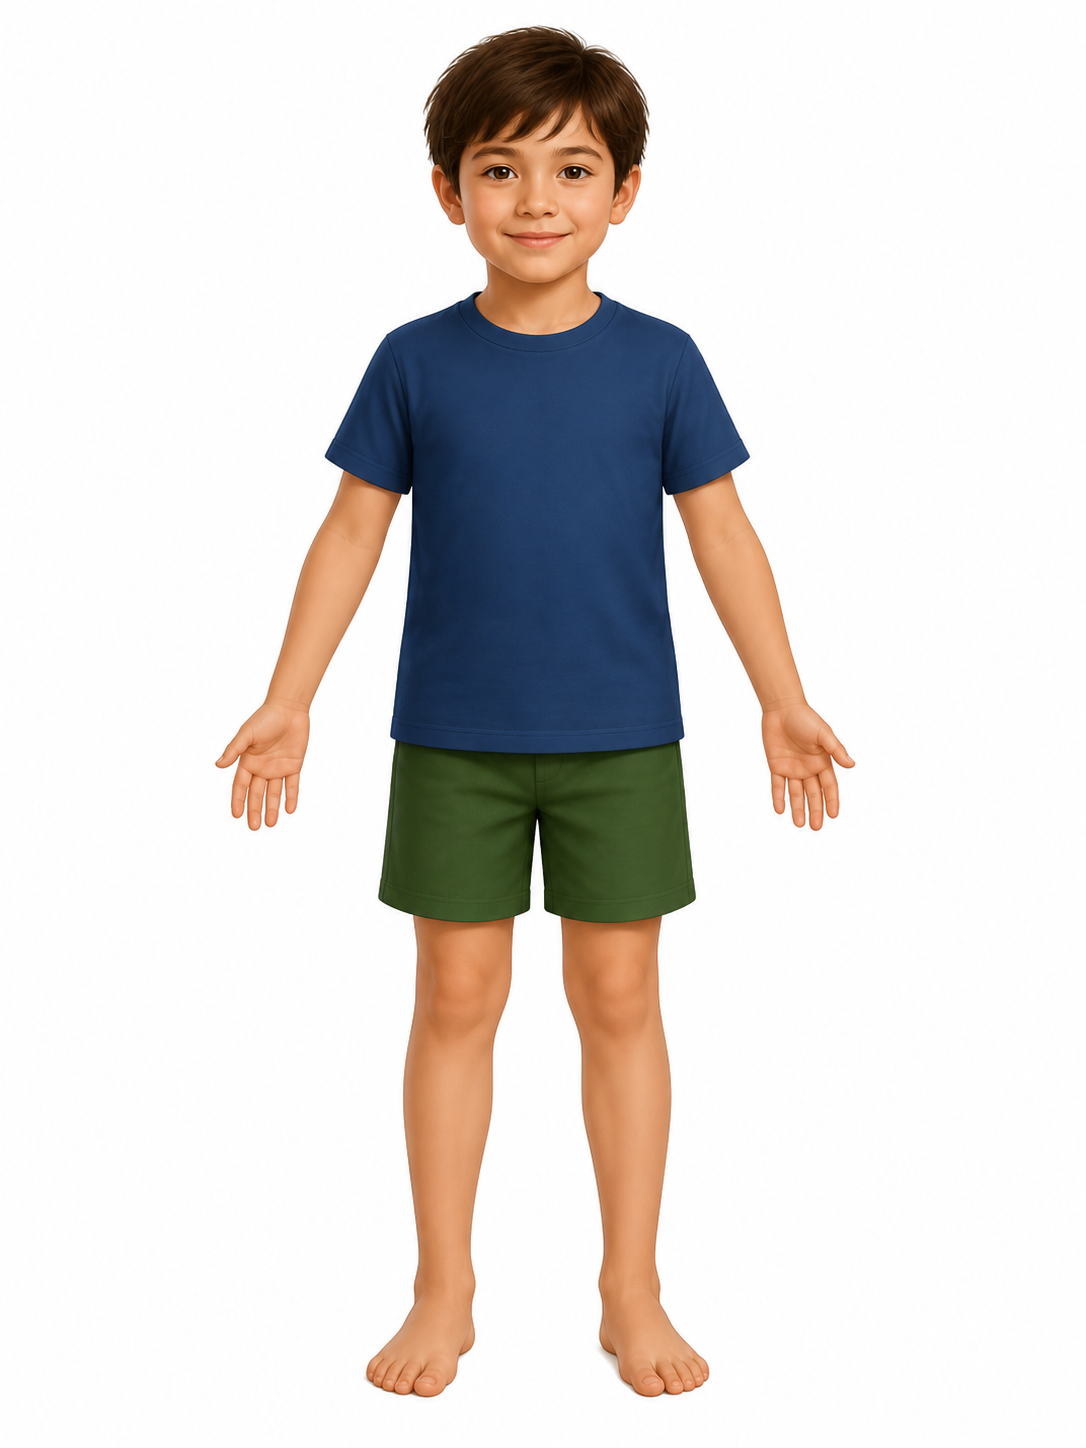
\includegraphics[width=0.42\linewidth]{images/book1/ai/fig-child-standing.png}};
  \begin{scope}[x={(img.south east)}, y={(img.north west)},
      every node/.style={font=\small}]
    \draw[omDef, thick] (0.57,0.90) -- (0.76,0.92) node[right] {सिर};
    \draw[omDef, thick] (0.53,0.80) -- (0.76,0.83) node[right] {गरदन};
    \draw[omDef, thick] (0.58,0.62) -- (0.78,0.66) node[right] {धड़};
    \draw[omDef, thick] (0.74,0.46) -- (0.86,0.38)
      node[below, align=center] {बाँह और\\ हाथ};
    \draw[omDef, thick] (0.60,0.18) -- (0.78,0.14)
      node[right, align=left] {टाँग और\\ पैर};
  \end{scope}
\end{tikzpicture}

{\small शरीर के तीन मुख्य भाग: \omterm{def:g1:my-body:parts}{सिर}, \omterm{def:g1:my-body:parts}{धड़} और चार \omterm{def:g1:my-body:parts}{उपांग} --- और गरदन, जो
\omterm{def:g1:my-body:parts}{सिर} को \omterm{def:g1:my-body:parts}{धड़} से जोड़ती है।}
\end{omfigure}

\begin{example}[बिल्ली जैसी ही बनावट?]\label{ex:g1:my-body:cat}
अपनी तुलना बिल्ली से करो: \omterm{def:g1:my-body:parts}{सिर}, \omterm{def:g1:my-body:parts}{धड़}, चार \omterm{def:g1:my-body:parts}{उपांग} --- बनावट एक जैसी लगती
है। पर बिल्ली चारों पर चलती है; तुम दो \omterm{def:g1:my-body:parts}{टाँगों} पर खड़े होते हो और दोनों
\omterm{def:g1:my-body:parts}{बाँहें} उठाने, चित्र बनाने और हाथ हिलाने के लिए ख़ाली रखते हो। और जहाँ
बिल्ली की पूँछ है, वहाँ तुम्हारे कुछ नहीं।
\end{example}

\section{मुड़ना: जोड़}

\begin{definition}[जोड़]\label{def:g1:my-body:joint}
\emph{जोड़}\index{जोड़} शरीर की वह जगह है जहाँ वह मुड़ या घूम सकता है।
\emph{कोहनी}\index{कोहनी} \omterm{def:g1:my-body:parts}{बाँह} को मोड़ती है, \emph{घुटना}\index{घुटना}
\omterm{def:g1:my-body:parts}{टाँग} को मोड़ता है, \emph{कंधा}\index{कंधा} पूरी \omterm{def:g1:my-body:parts}{बाँह} को घुमाता है,
और \emph{कलाई}\index{कलाई} तथा \emph{टखना}\index{टखना} हाथ और पैर को
मोड़ते हैं। दो जोड़ों के बीच शरीर सीधा ही रहता है।
\end{definition}

\begin{omfigure}
\begin{tikzpicture}[scale=1.0]
  % straight arm
  \draw[very thick] (0,0) -- (2.0,0);
  \draw[very thick] (2.0,0) -- (3.8,0);
  \fill[omThm] (2.0,0) circle (0.1);
  \fill[omDef!60] (0,0) circle (0.1);
  \draw[thick, fill=omDef!8] (4.0,0) circle (0.18);
  \node[below, font=\small] at (1.9,-0.3) {सीधी रखी बाँह};
  % bent arm
  \begin{scope}[xshift=6.6cm]
    \draw[very thick] (0,0) -- (2.0,0);
    \draw[very thick] (2.0,0) -- (3.1,1.45);
    \fill[omThm] (2.0,0) circle (0.1);
    \fill[omDef!60] (0,0) circle (0.1);
    \draw[thick, fill=omDef!8] (3.22,1.6) circle (0.18);
    \node[below, font=\small] at (1.9,-0.3) {कोहनी से मुड़ी बाँह};
    \draw[omThm] (2.05,0.12) -- (1.55,0.8)
      node[above left, font=\small, omThm] {जोड़ मुड़ता है};
  \end{scope}
  \node[font=\small] at (1.0,1.4) {कंधा};
  \draw[omDef!60] (0.05,0.12) -- (0.55,1.15);
\end{tikzpicture}

{\small \omterm{def:g1:my-body:parts}{बाँह} सिर्फ़ अपने जोड़ों पर मुड़ती है: \omterm{def:g1:my-body:joint}{कंधा} (नीला) और \omterm{def:g1:my-body:joint}{कोहनी}
(लाल)। इनके बीच वह सीधी ही रहती है।}
\end{omfigure}

\begin{example}[करके देखो: अकड़े घुटनों की चाल]\label{ex:g1:my-body:stiff}
घुटने मोड़े बिना चलकर देखो। बस किसी तरह चल तो जाता है --- बत्तख़ जैसे
अकड़े छोटे-छोटे क़दमों से। अब घुटने, कूल्हे या पीठ मोड़े बिना फ़र्श से
पेंसिल उठाकर देखो। \omterm{def:g1:my-body:joint}{जोड़} ही शरीर की हरकतों को चिकना, तेज़ और आसान बनाते
हैं।
\end{example}

\begin{remark}[दायाँ और बायाँ]\label{rem:g1:my-body:sides}
शरीर के दो पहलू हैं, दायाँ और बायाँ, लगभग आईने जैसे: हर तरफ़ एक \omterm{def:g1:my-body:parts}{बाँह}
और एक \omterm{def:g1:my-body:parts}{टाँग}, \omterm{def:g1:my-body:parts}{सिर} के हर तरफ़ एक आँख और एक कान। अपना दायाँ हाथ बाएँ से
पहचानना भी शरीर की ही जानकारी है --- इसी से लोग समझते हैं कि तुम किस
ओर की बात कर रहे हो।
\end{remark}

\section{मेरा शरीर बढ़ता है}

\begin{proposition}[बड़े होना]\label{prop:g1:my-body:growth}
बच्चे का शरीर \emph{बढ़ता है}\index{बढ़ना}: वह साल-दर-साल लंबा और भारी
होता जाता है, जब तक बड़ों का क़द न पा ले। बढ़ना धीमा और लगातार होता है
--- महसूस करने के लिए बहुत धीमा, नापने के लिए बहुत आसान।
\end{proposition}
\admitted

\begin{example}[दरवाज़े की चौखट पर निशान]\label{ex:g1:my-body:doorframe}
चौखट से सटकर खड़े हो जाओ; कोई बड़ा पेंसिल से तुम्हारे क़द का निशान
लगाता है। कुछ महीनों बाद फिर ऐसा करो: नया निशान ऊपर है! तुमने अपने
आपको बढ़ते हुए कभी महसूस नहीं किया, पर एक के ऊपर एक लगे ये दो निशान
इसे साफ़ दिखा देते हैं।
\end{example}

\begin{omfigure}
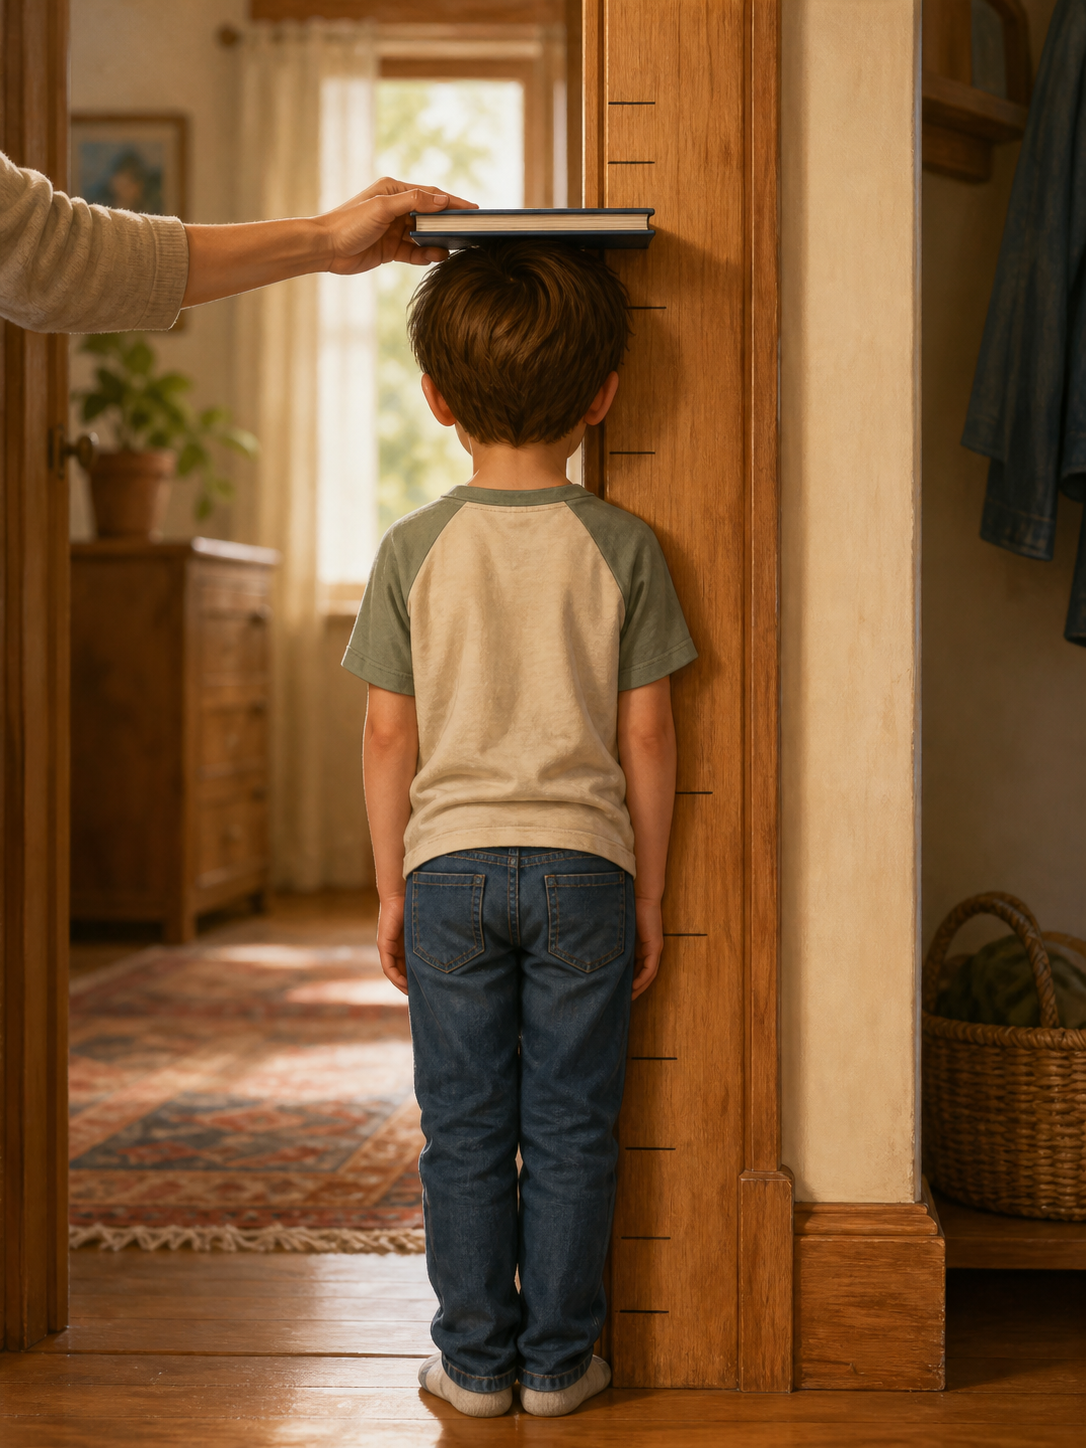
\includegraphics[width=0.46\linewidth]{images/book1/ai/g1-body-doorframe.png}

{\small चौखट पर नापने का दिन: चपटी किताब \omterm{def:g1:my-body:parts}{सिर} की सबसे ऊँची जगह को
सीधे लकड़ी तक ले आती है।}
\end{omfigure}

\begin{method}[अपना क़द नापना]\label{met:g1:my-body:measure}
\begin{enumerate}
  \item अपने जूते उतारो;
  \item सीधे खड़े हो जाओ, पीठ और एड़ियाँ दीवार से सटी हों, नज़र सामने
        हो;
  \item कोई मददगार तुम्हारे \omterm{def:g1:my-body:parts}{सिर} पर एक चपटी किताब रखे, समतल, दीवार को
        छूती हुई;
  \item किताब के नीचे की जगह पर निशान लगाओ, और उसके बग़ल में तारीख़
        लिखो।
\end{enumerate}
हर बार एक ही तरीक़े से नापे गए निशानों पर भरोसा किया जा सकता है ---
और उनकी तुलना भी की जा सकती है।
\end{method}

\begin{remark}[हर शरीर अलग है]\label{rem:g1:my-body:different}
एक ही कक्षा में कुछ बच्चे लंबे होते हैं, कुछ नाटे; कुछ पहले बढ़ते हैं,
कुछ बाद में। यह सब सामान्य है। शरीर चेहरों जैसे हैं: एक ही बनावट पर
बने, और हर एक अलग। तुम्हारी चौखट के निशान तुम्हारे हैं --- वे पड़ोसी
से होड़ लगाने के लिए नहीं हैं।
\end{remark}

\section{अभ्यास}

\begin{exercise}[$\star$]\label{exo:g1:my-body:1}
मानव शरीर के तीन मुख्य भागों के नाम बताओ। \omterm{def:g1:my-body:parts}{सिर} को \omterm{def:g1:my-body:parts}{धड़} से क्या जोड़ता
है?
\end{exercise}

\begin{exercise}[$\star$]\label{exo:g1:my-body:2}
हर \omterm{def:g1:my-body:parts}{उपांग} कहाँ ख़त्म होता है --- \omterm{def:g1:my-body:parts}{बाँह} के सिरे पर क्या है, और \omterm{def:g1:my-body:parts}{टाँग} के
सिरे पर?
\end{exercise}

\begin{exercise}[$\star$]\label{exo:g1:my-body:3}
कौन-सा \omterm{def:g1:my-body:joint}{जोड़} मोड़ता है: (क) \omterm{def:g1:my-body:parts}{बाँह} को बीच से? (ख) \omterm{def:g1:my-body:parts}{टाँग} को बीच से? (ग)
\omterm{def:g1:my-body:parts}{बाँह} के सिरे पर हाथ को?
\end{exercise}

\begin{exercise}[$\star$]\label{exo:g1:my-body:4}
अपने बाएँ हाथ से अपना दायाँ कान छुओ। तुम्हारी \omterm{def:g1:my-body:parts}{बाँह} ने अभी कौन-कौन से
\omterm{def:g1:my-body:joint}{जोड़} इस्तेमाल किए? कम से कम दो बताओ।
\end{exercise}

\begin{exercise}[$\star$]\label{exo:g1:my-body:5}
\cref{ex:g1:my-body:cat} में एक बात ढूँढ़ो जिसमें तुम्हारा शरीर
बिल्ली जैसा है और दो बातें जिनमें अलग है।
\end{exercise}

\begin{exercise}[$\star$]\label{exo:g1:my-body:6}
\cref{met:g1:my-body:measure} में मददगार सिर्फ़ देखने के बजाय \omterm{def:g1:my-body:parts}{सिर} पर
चपटी किताब क्यों रखता है?
\end{exercise}

\begin{exercise}[$\star$]\label{exo:g1:my-body:7}
चौखट पर दो निशान: पिछले साल का, और आज का थोड़ा ऊपर। ये निशान क्या
दिखाते हैं? क्या तुमने इसे होते हुए महसूस किया?
\end{exercise}

\begin{exercise}[$\star$]\label{exo:g1:my-body:8}
करके देखो: \cref{ex:g1:my-body:stiff} वाली अकड़े घुटनों की चाल चलो,
फिर \omterm{def:g1:my-body:joint}{कोहनियाँ} मोड़े बिना ताली बजाकर देखो। रोज़ की कौन-सी हरकतों में
जोड़ों की ज़रूरत निकल आती है?
\end{exercise}

\begin{exercise}[$\star\star$]\label{exo:g1:my-body:9}
मीरा अपनी कक्षा में सबसे छोटी है और इससे परेशान है।
\cref{rem:g1:my-body:different} उसे क्या उत्तर देता है?
\end{exercise}

\begin{exercise}[$\star\star$]\label{exo:g1:my-body:10}
लकड़ी की एक ही छड़ से बनी कठपुतली कुर्सी पर नहीं बैठ सकती। तुम छड़ को
कहाँ काटकर घूमने वाले बिंदु जोड़ोगे ताकि वह बैठ सके? बताओ कि तुम्हारे
कट शरीर के कौन-से जोड़ों की नक़ल हैं।
\end{exercise}
